\documentclass[10pt,a4paper]{article}
\usepackage[utf8]{inputenc}
\usepackage{amsmath}
\usepackage{amsfonts}
\usepackage{amssymb}
\usepackage{graphicx}
\usepackage{enumerate}
\begin{document}

\section{Set Theory}

To demystify mathematics consider
\begin{enumerate}[(i)]
\item What is a theorem?
\item What is a proof?
\end{enumerate}
What if we don't know the answer?

To begin we need
\begin{enumerate}[(a)]
\item an example(s)
\item a nearly related concept
\end{enumerate}


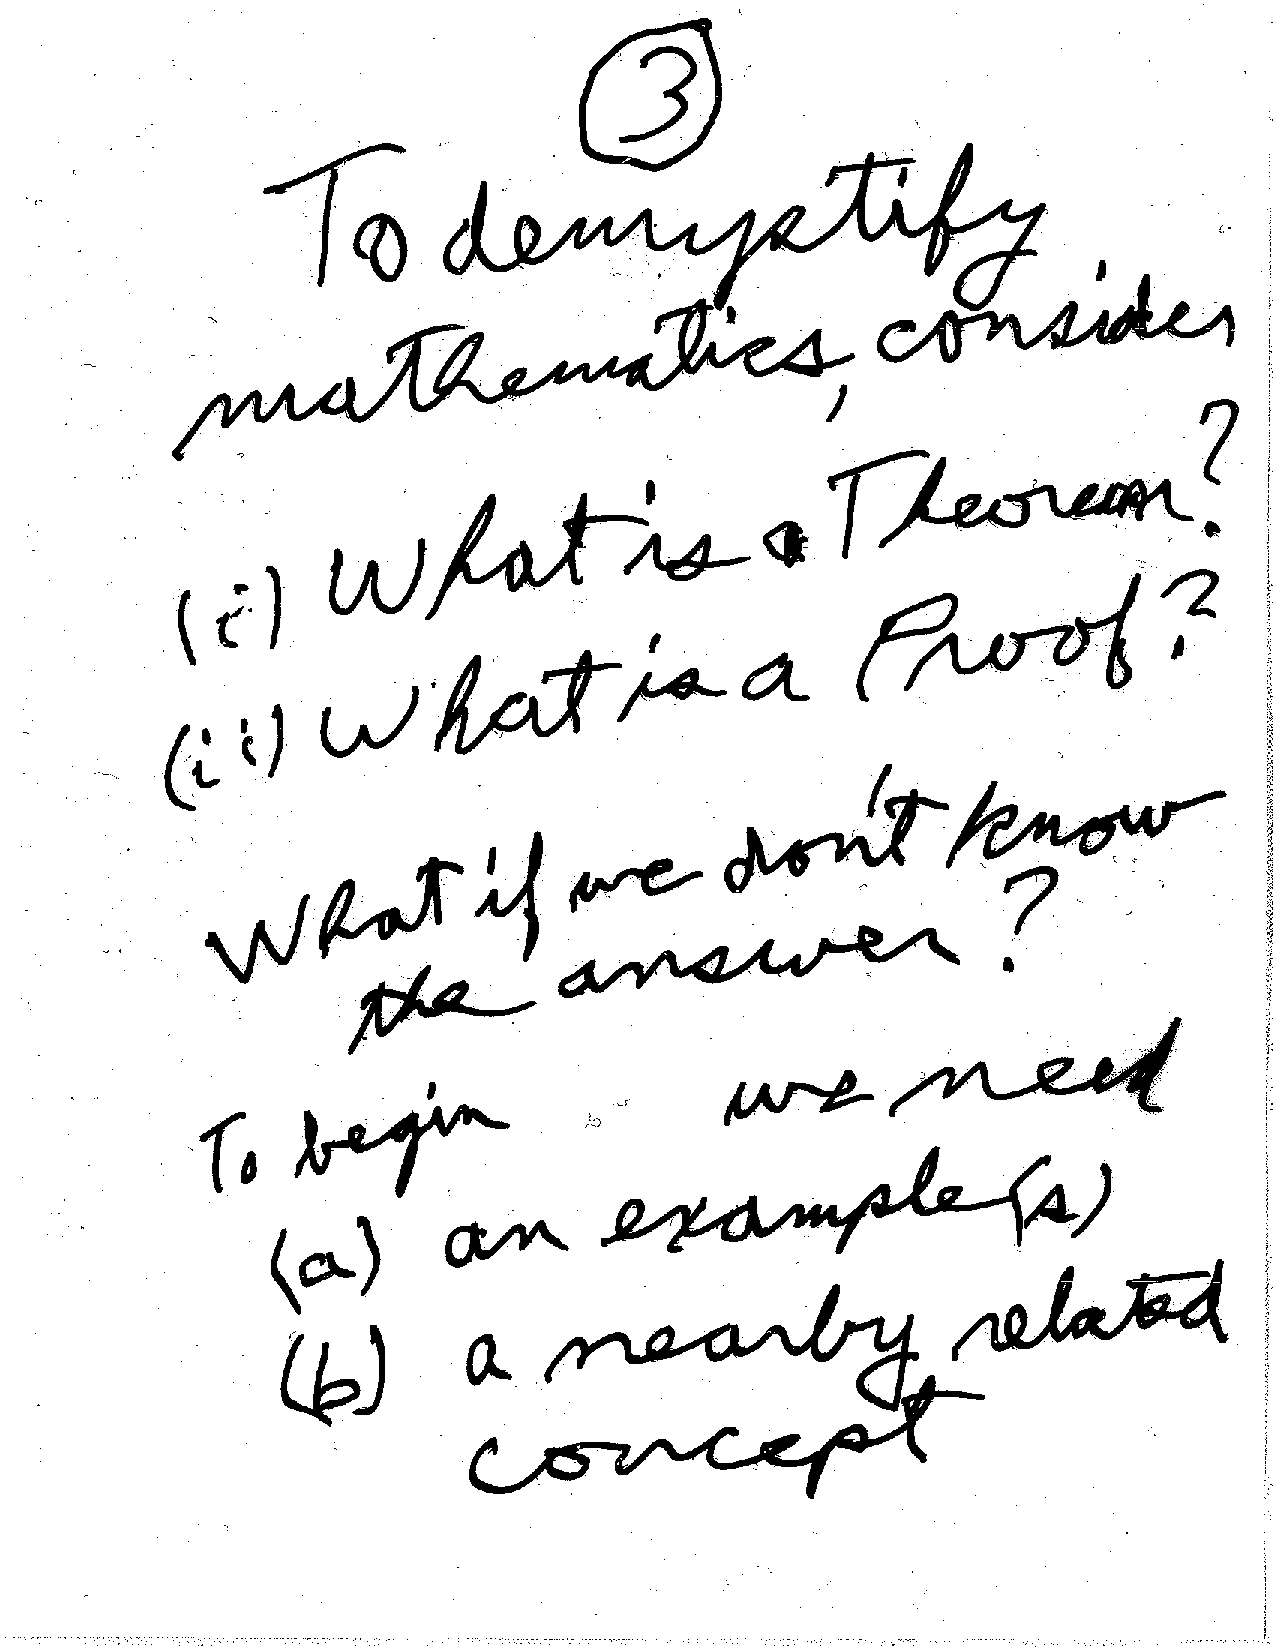
\includegraphics[scale=.5]{Pages/ST_3}

\newpage

Related Concept: Greek Syllogism

\underline{example:}
\begin{enumerate}
\item All men are mortal.
\item Socrates is a man.
\item Therefore, Socrates must die. 
\end{enumerate}

To analyze, recast in set theoretic terms via Venn Diagram.

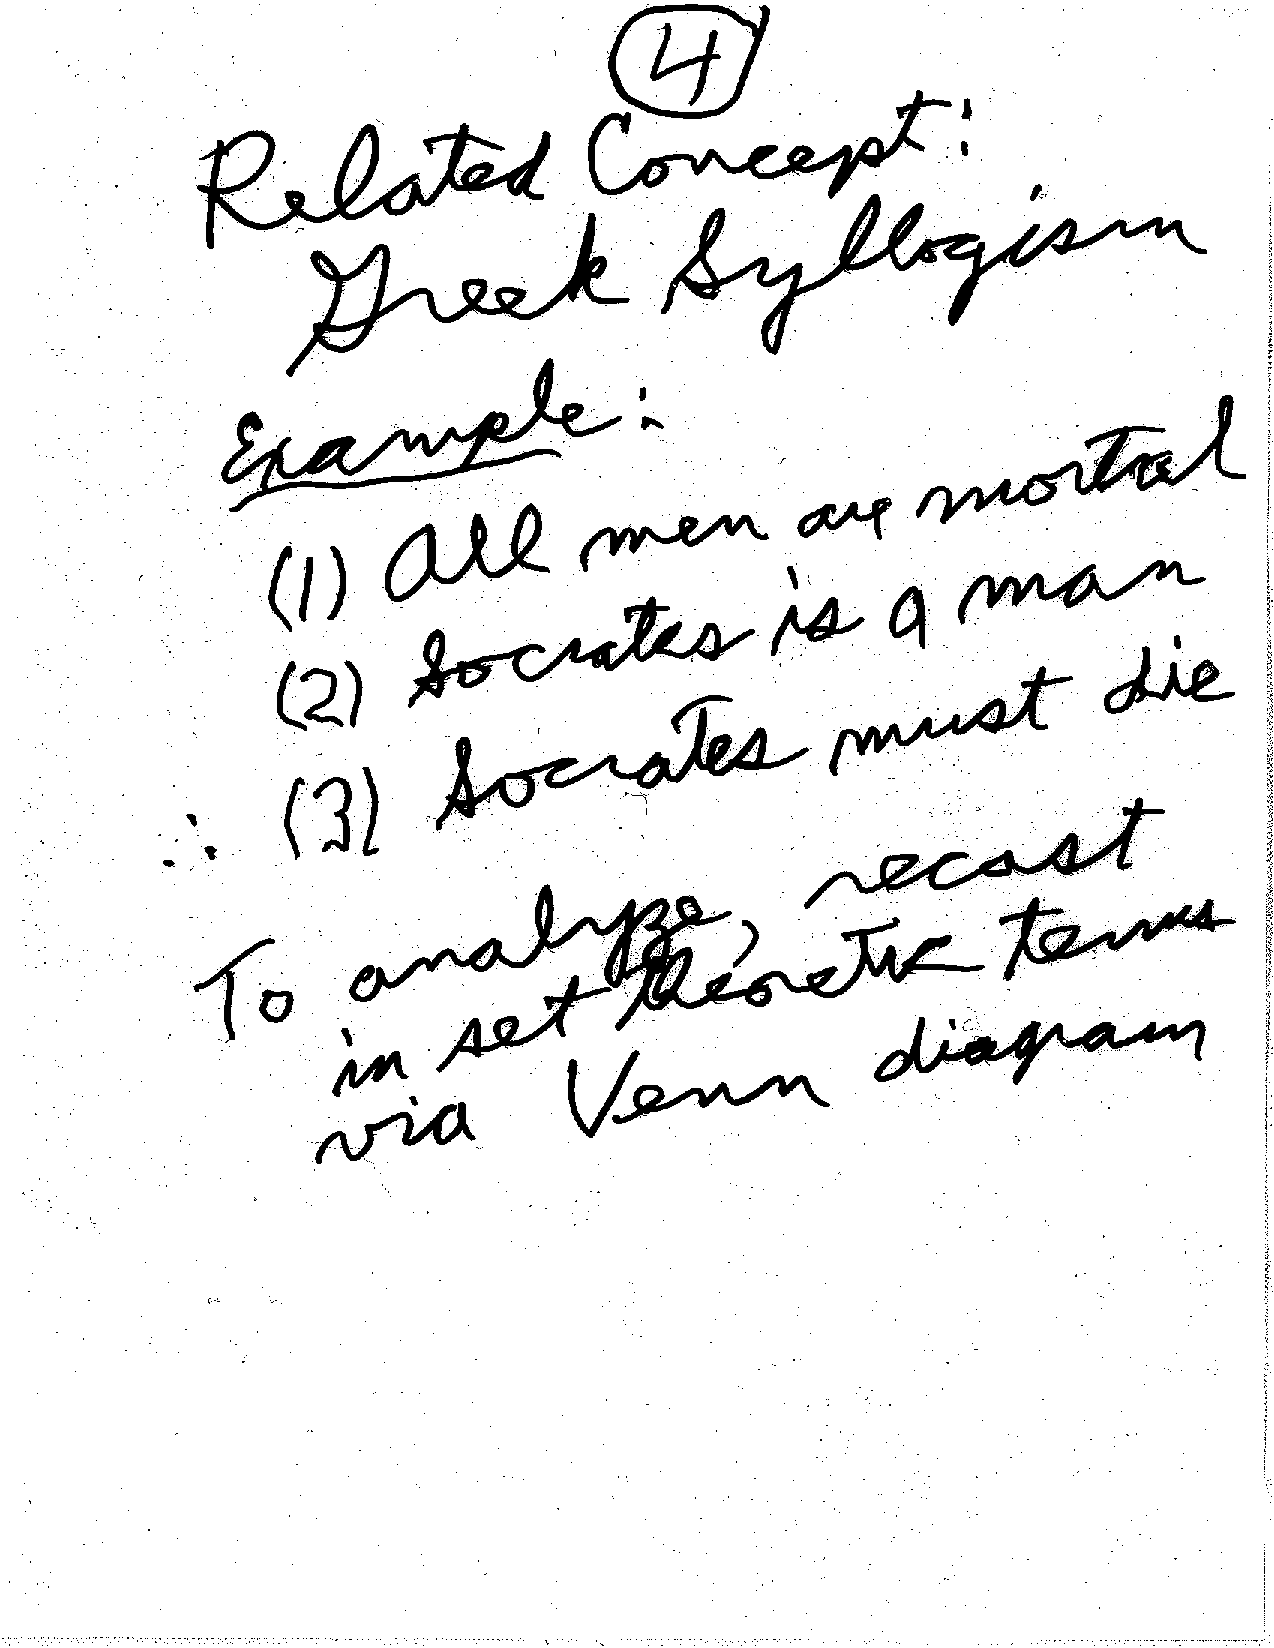
\includegraphics[scale=.5]{Pages/ST_4}

\newpage

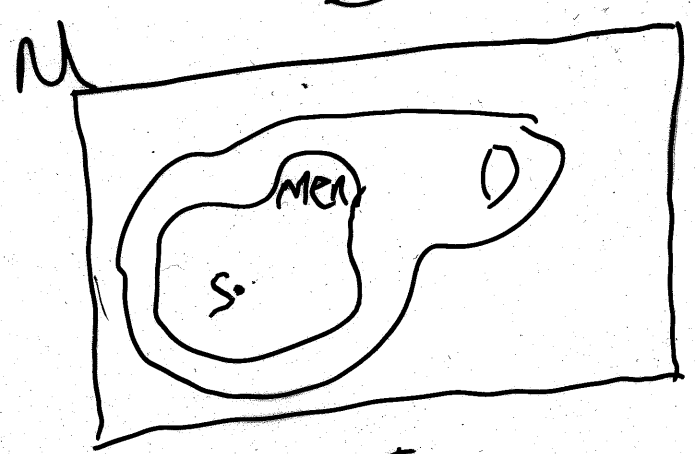
\includegraphics[scale=.2]{Pages/ST_5_im1}

$S$: Socrates\\
$M$: Set of Men\\
$D$: Things that will die\\
$\mathcal{U}$: Things on Earth

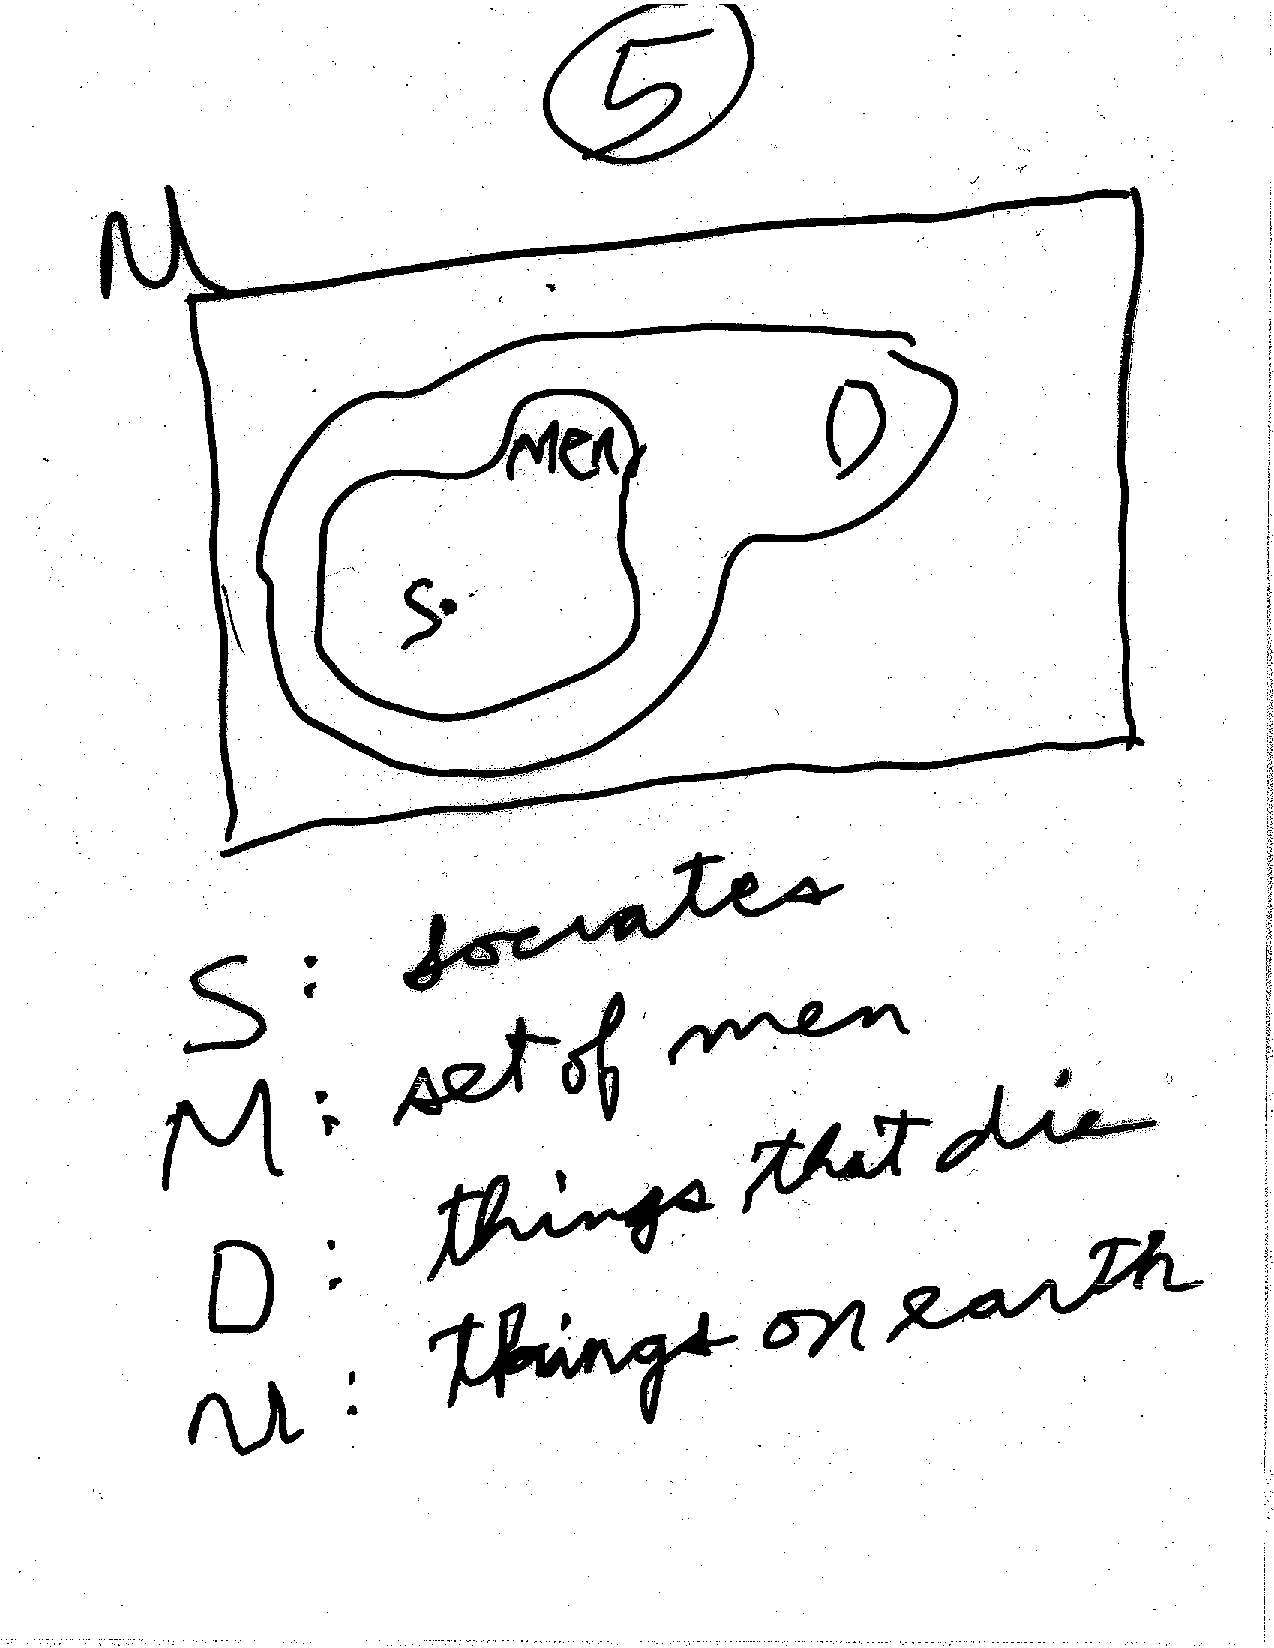
\includegraphics[scale=.5]{Pages/ST_5} 



%Zack: Pages 6,7,8,19,20

%Jack: 21, 9, 10, 11

%Koka: Pages 13, 13A, 22 ,22A, 22B


\section{Generate $\mathbb{N}$}


%Ruth: Pages L4A-L4G




\section{From $\mathbb{Z}$ to $\mathbb{R}$ via ordering}
%Jazz: ZR1-ZR5

%Kyler: ZR6 - ZR10

%Preethika: ZR11-ZR14


\section{Sequence and Limits}

%Aaron: First 2 pages and 48-50

%Hamza: 51-52B

\section{Limit and Convergence}

%Joe: 50-51

%Quinten: 52-53

%Farishta: 53A-54A

\section{Infinite Series}

%Sukhreet: IS1 - IS 7

%Matthew: IS8 - IS15

%Will: IS16 - IS23

%Rebecca: IS24 - IS32

%Maady: IS33 - IS42

\section{Metric Spaces Part 1}

%Travis: M1 - M5

%Jerome: M6- M10
\newpage
for any z $\epsilon$ m the path $x \rightarrow z$ followed by $z \rightarrow y$ can be no shorter than the shortest path from $x$ to $y$ hence we require $$(iv)d (\frac{x}{y}) \leq d(x,z) + d(z,y)$$ This is called the triangle inequality.
 
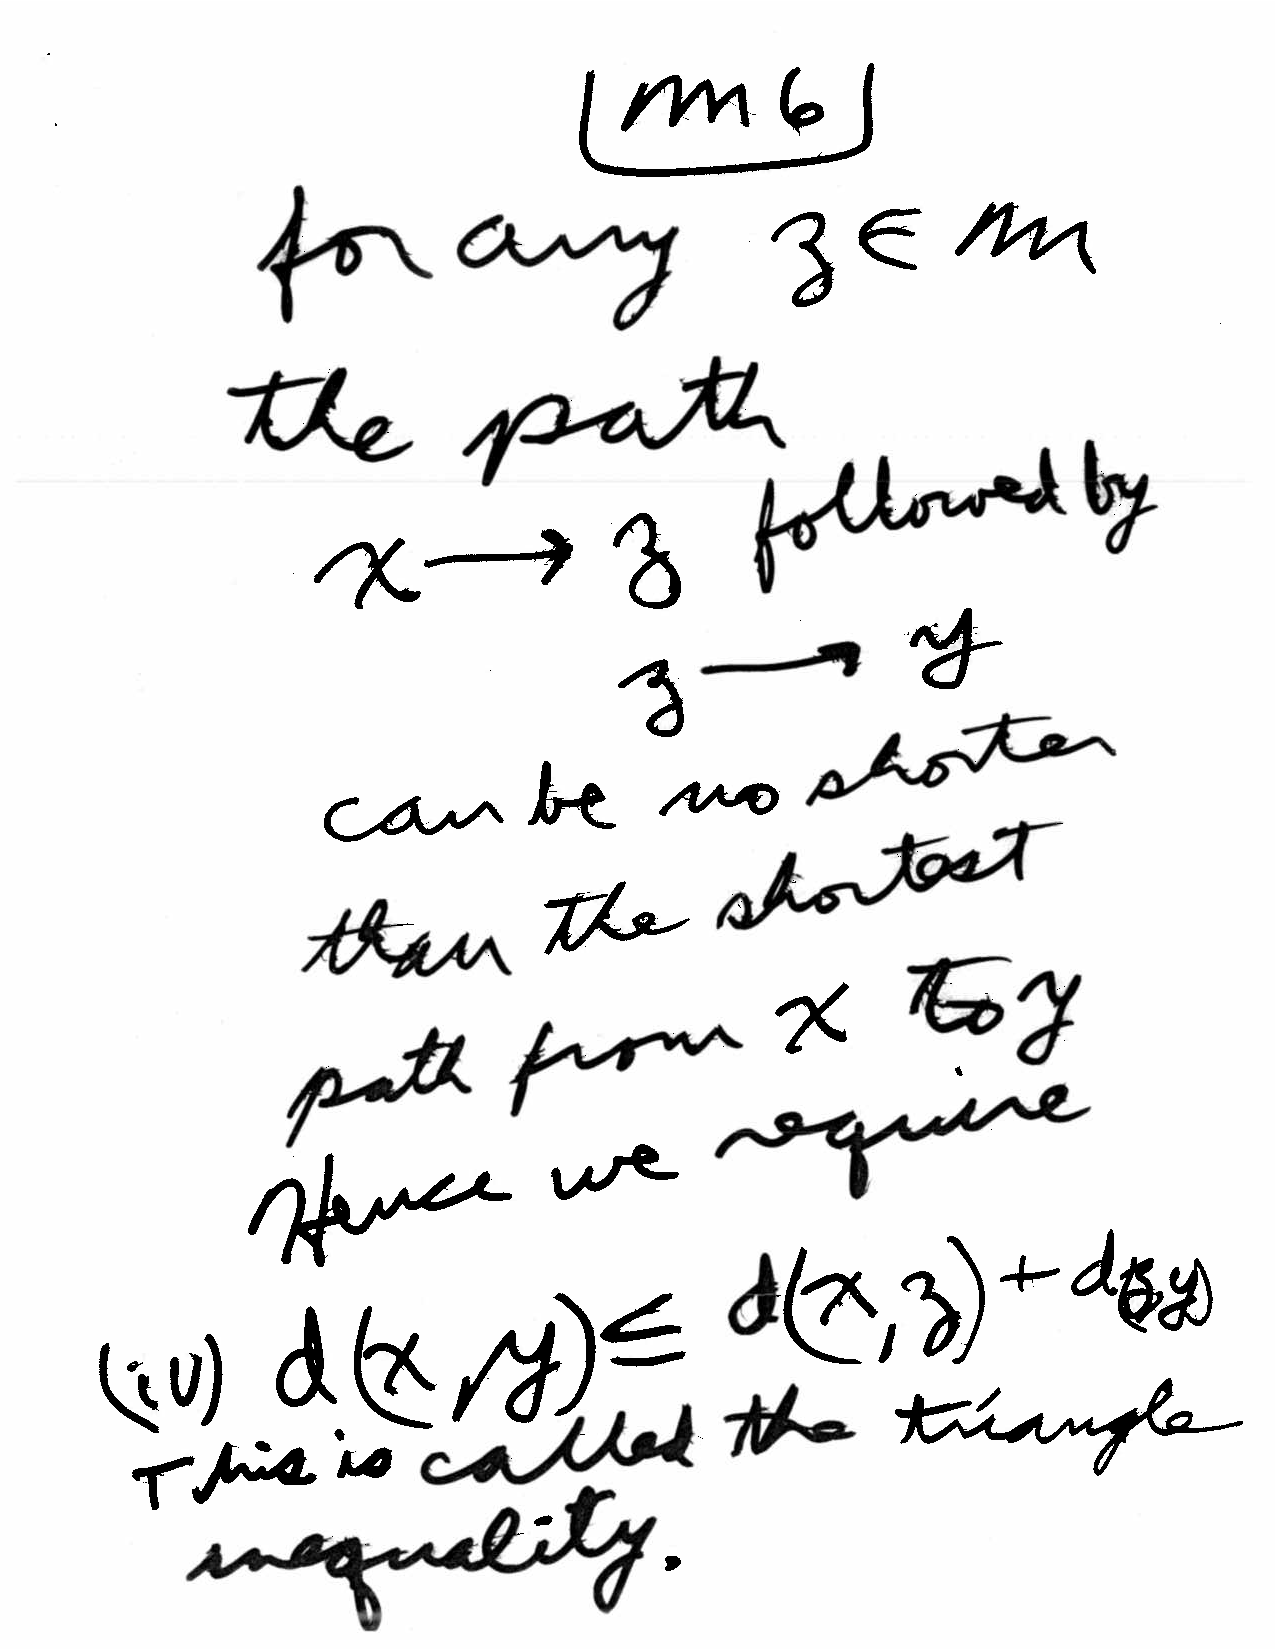
\includegraphics[scale=.5]{Pages/MS_6}

\newpage

\underline{Def}: Any d: $m \times m \rightarrow [0,\infty)$ satisfying conditions $(i) - (iv)$ will be called a \underline{metric} on $m$. How could we construct a metric? Suppose $m$ is a finite set of points. Thinking of these as cities in a given state / region. 

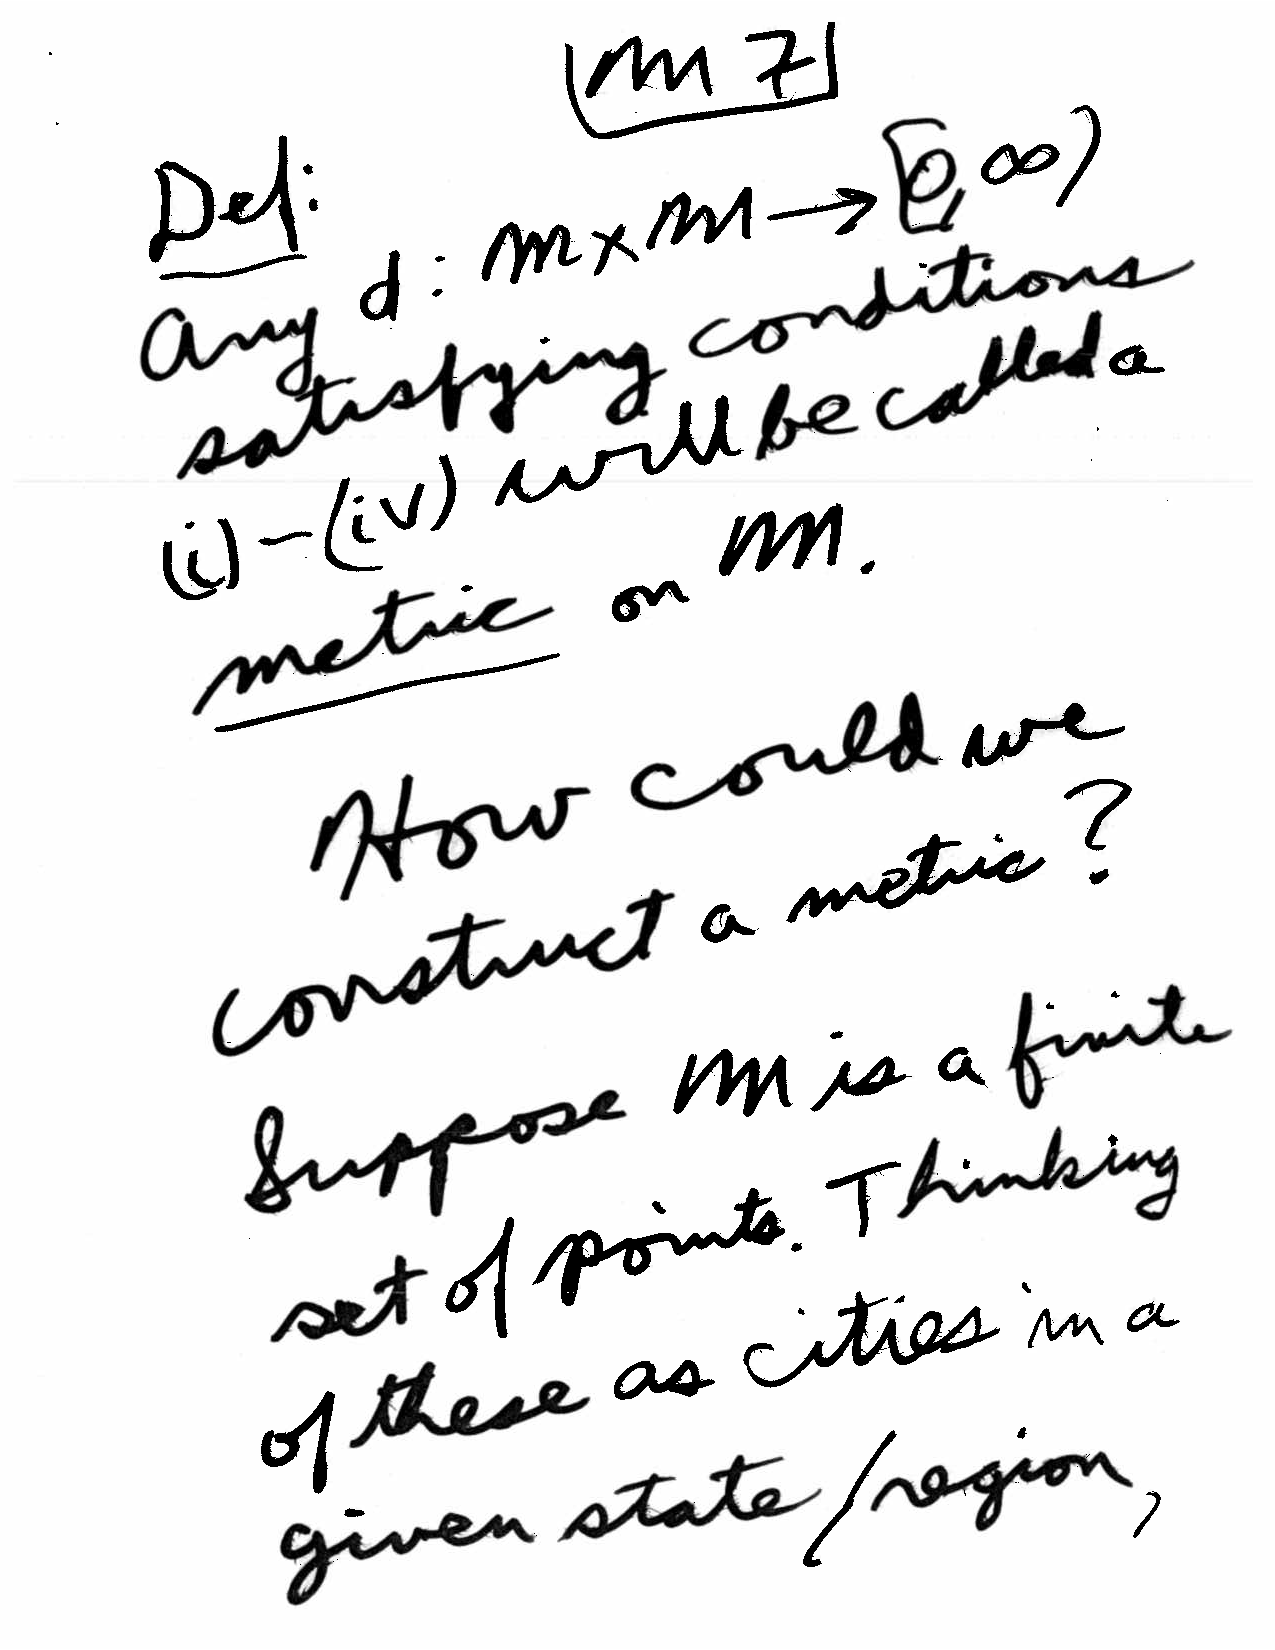
\includegraphics[scale=.5]{Pages/MS_7}

\newpage

Call them $ C_1 , C_2 , \ldots , C_L $ Suppose some pairs $(i,j)$ of cities $C_i$ and $C_j$ are adjacent in that they are linked by a non-stop road of some positive, finite, known distance. $g_{ij}$. When is there a path by car between every two cities? 
 
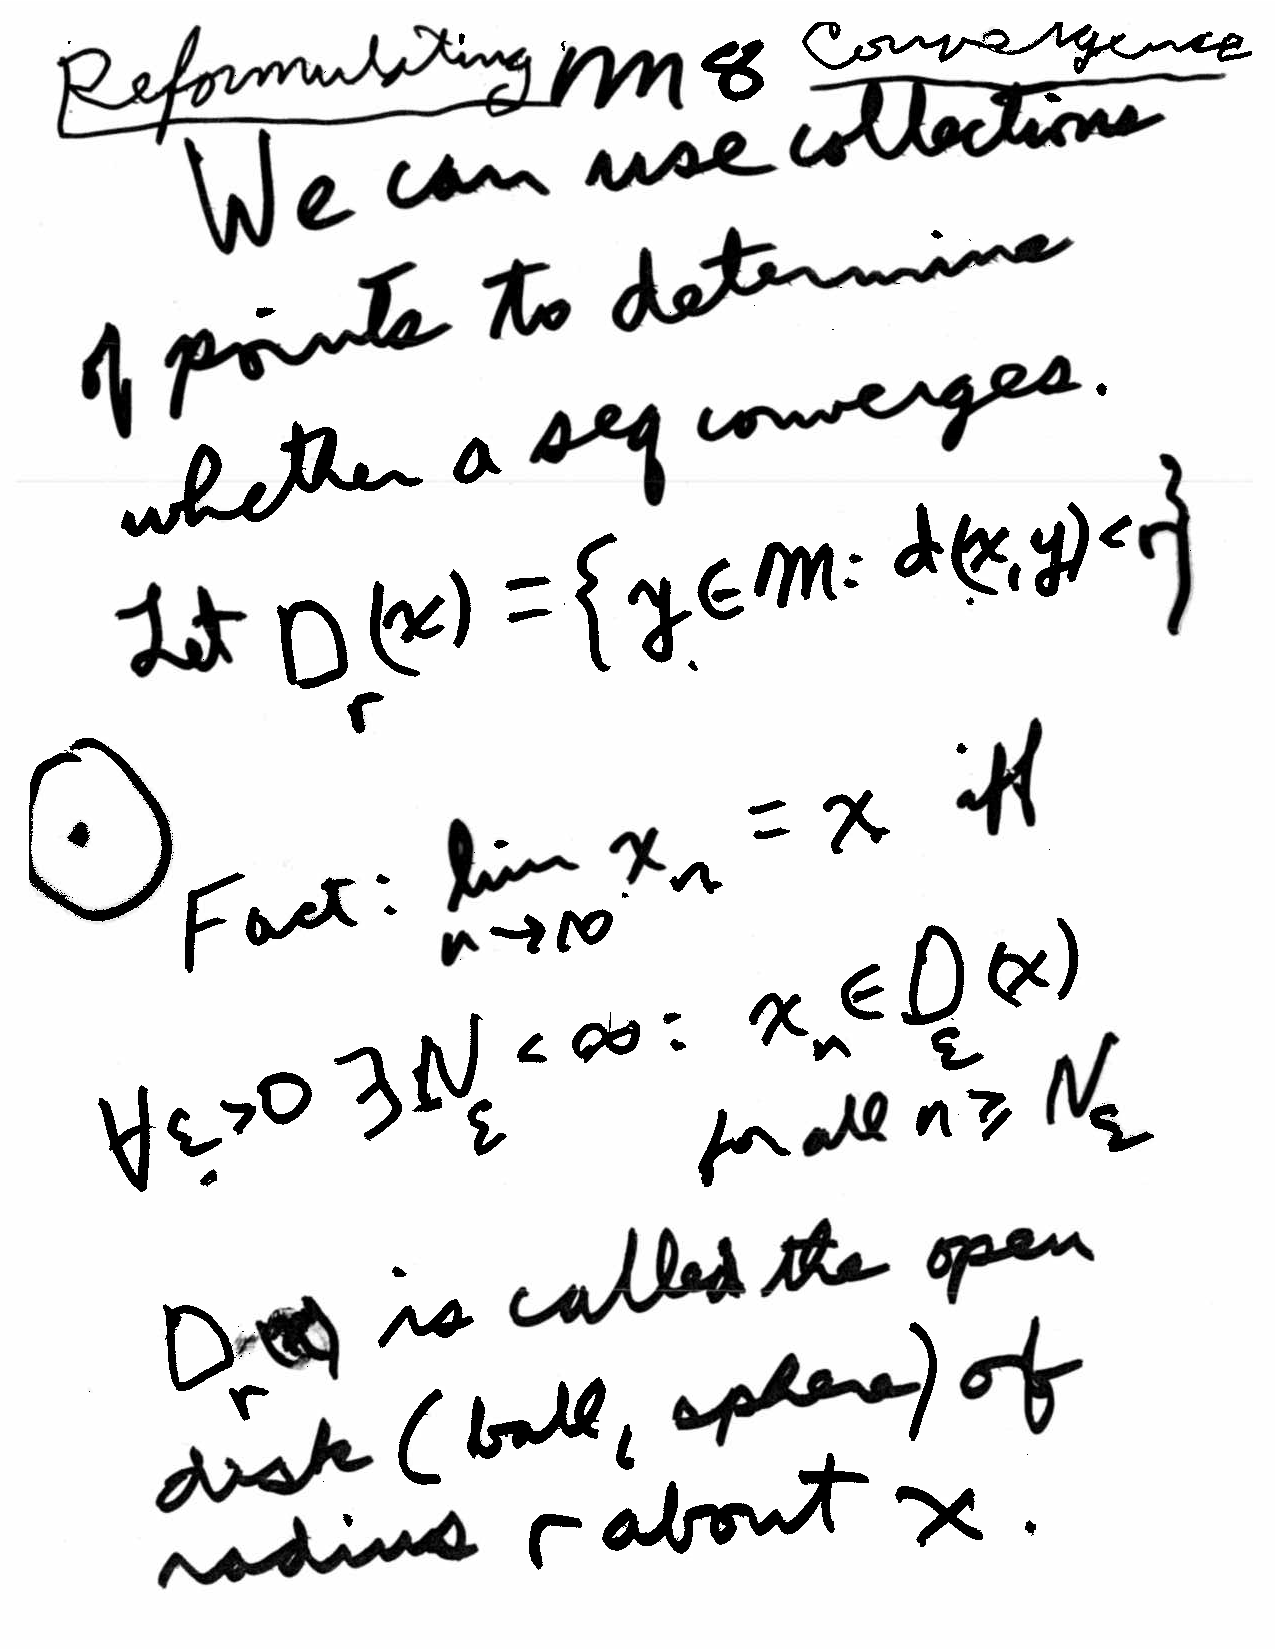
\includegraphics[scale=.5]{Pages/MS_8}

\newpage

\underline{Ans.} \newline
Let $A = (a_{ij} )$ be an $L x L$ incidence matrix where $$ a_{ii} \equiv 1  \mbox{ and for } i \neq j$$ 
$$a_{ij} = 
\begin{cases} 
1 & \mbox{ if } C_i \mbox{ and } C_j \mbox{ are adjacent } \\ 
0 & \mbox{ otherwise }
\end{cases}$$ \newline
Let $A^k \equiv (a_{ij_{j^k}})$ $$a_{ij_{j^k}} > 0$$ iff there is a path along adjacent cities between $C_i$ and $C_j$ taking at most $k$ steps. 

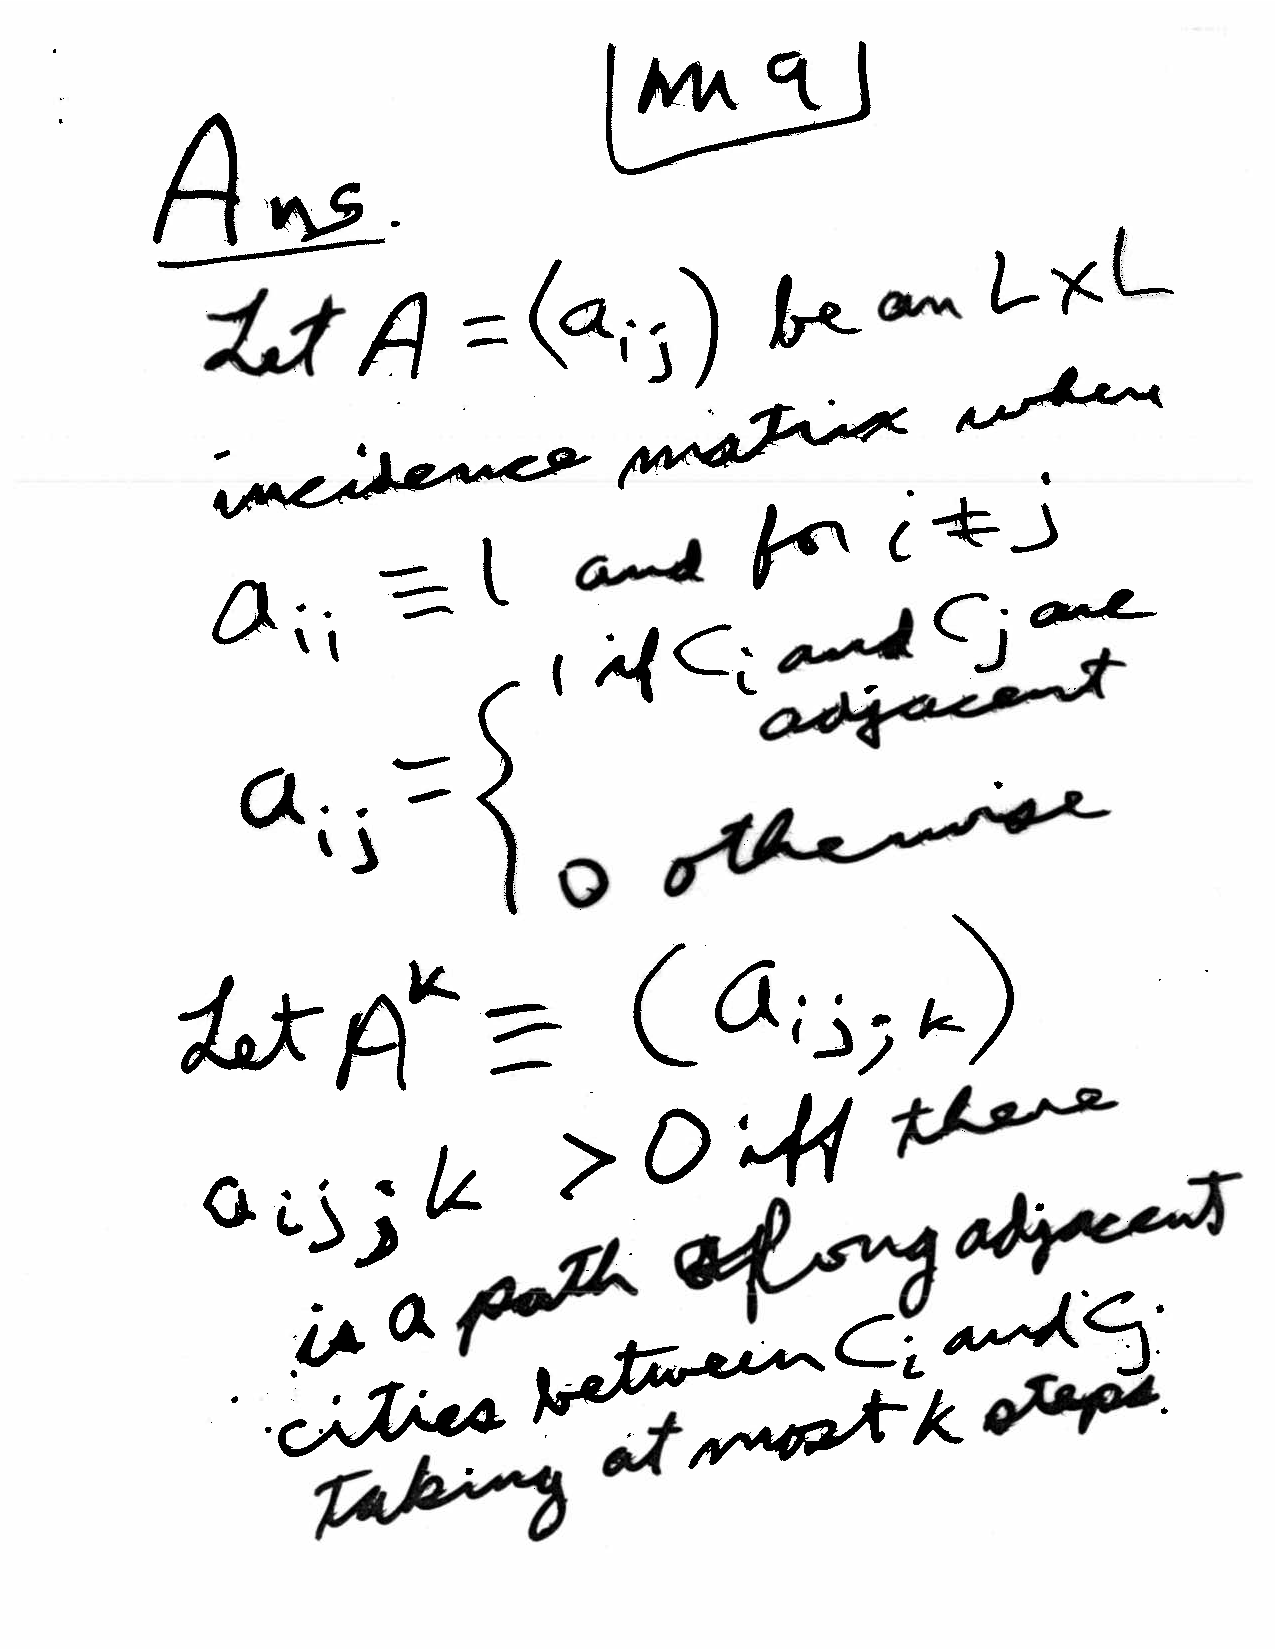
\includegraphics[scale=.5]{Pages/MS_9}


\newpage

Hence transportation by car is feasible between any two cities iff $a_{ij_{j^{l-1}}} > 0$ for all $1 \leq i,j \leq L-1$ The distance $d(C_i, C_j)$ would then be define as the sum of the length producing the shortest path. 

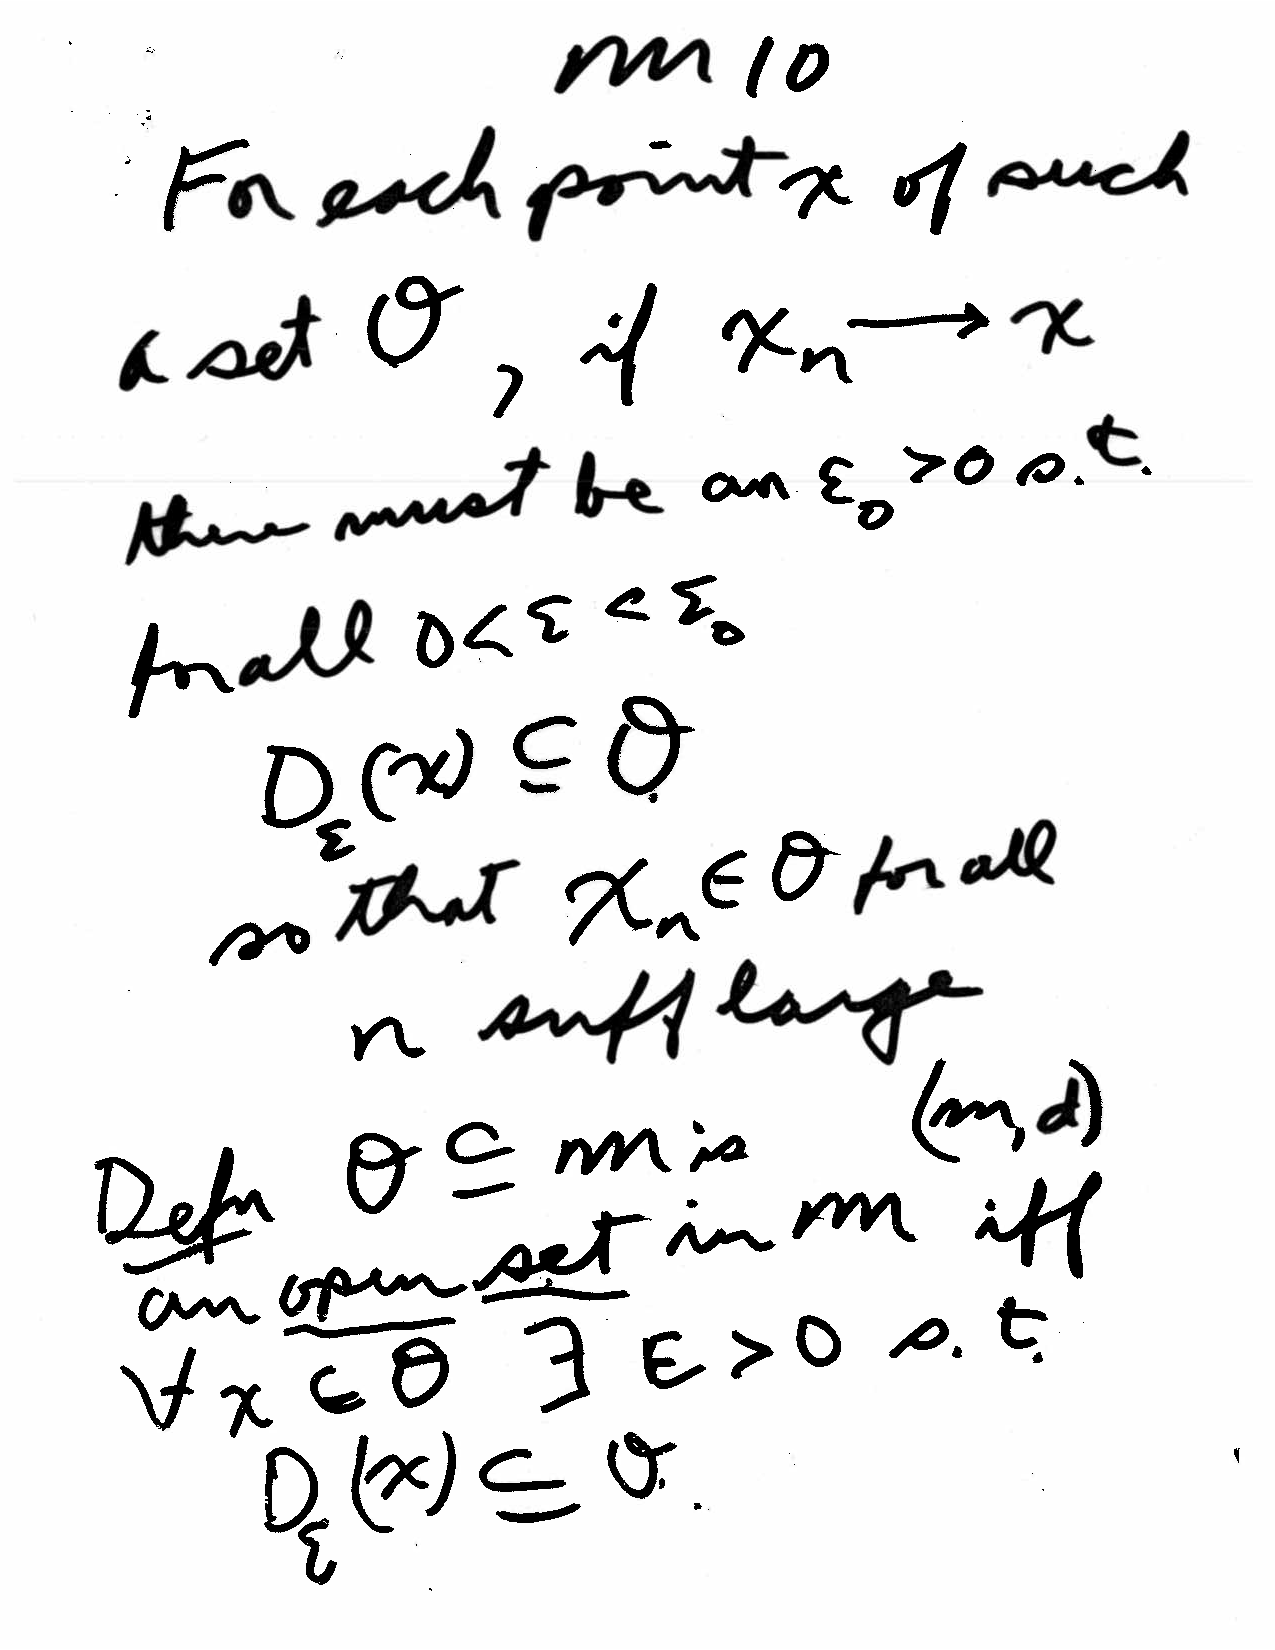
\includegraphics[scale=.5]{Pages/MS_10}

%Jerome: IS40-IS42

\newpage

Then 
$$h_n (x) \equiv f_n (x) g_n (x) \rightarrow h(x)$$ Notice that
$$h_n (x) = \sum_{j=0}^{2n} a_nx^j \sum_{k=0}^n b_kx^k$$ $$= \sum_{r=0}^{2n} (\sum_{j=0}^r a_jb_{r-j})x^r$$ $$+ \sum_{ \{ 0 \leq j, k \leq 2n : j+k > 2n\}} a_jb_kx^{j+k}$$ $$\equiv \tilde{h}_n(x) + \gamma_n(x)$$

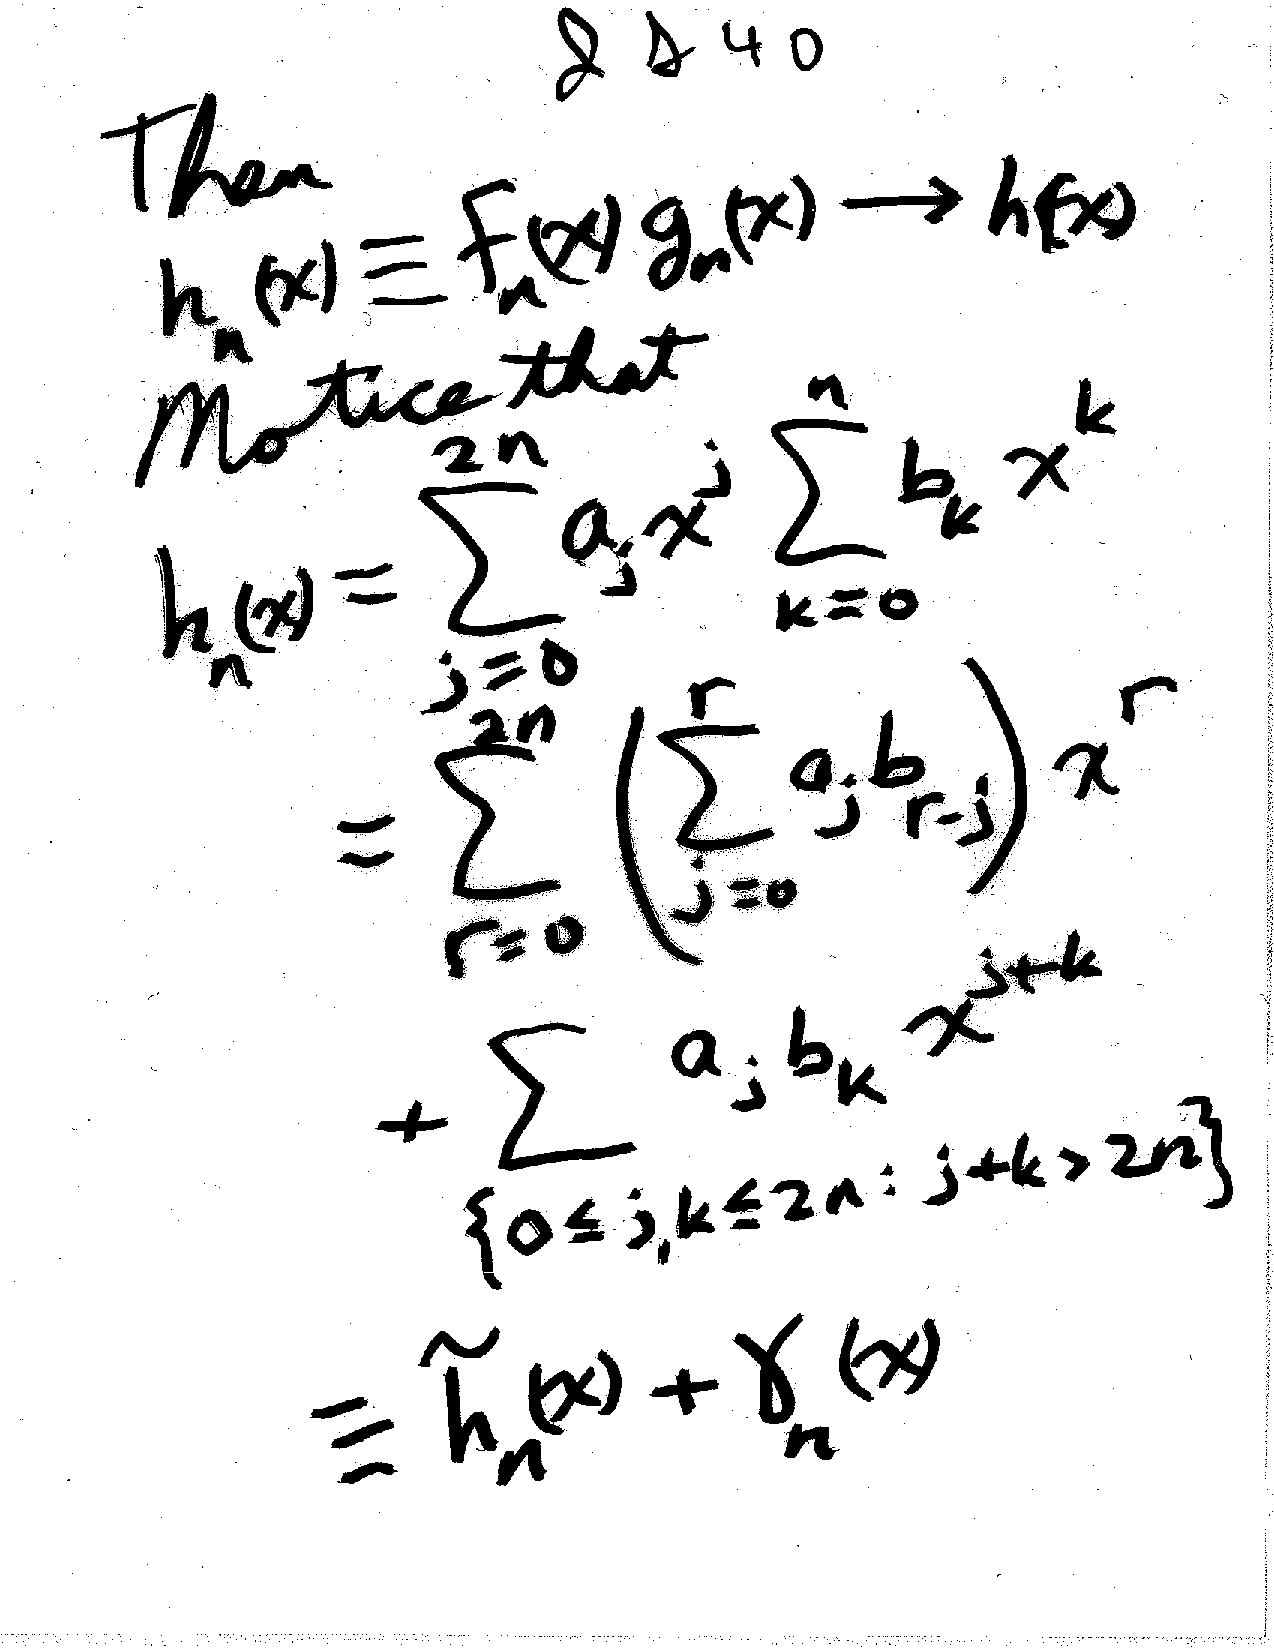
\includegraphics[scale=.5]{Pages/IS_40}

\newpage 

For $n \geq j_*$,
$$|\gamma_n (x)| \leq \sum_{j=0}^n |a_jx^j| \sum_{k=n+1}^\infty |b_kx^k|$$ 
$$+  \sum_{j=n+1}^\infty |a_jx^j| \sum_{k=0}^n |b_kx^k|$$ $$\leq F(x) \sum_{k=n+1}^\infty \lambda^k$$ $$+ G(x)
\sum_{j=n+1}^\infty \lambda^j$$ $$= \frac{(F(x)+G(x)\lambda^{n+1}}{1-\lambda} \rightarrow 0 $$ as $n \rightarrow \infty$

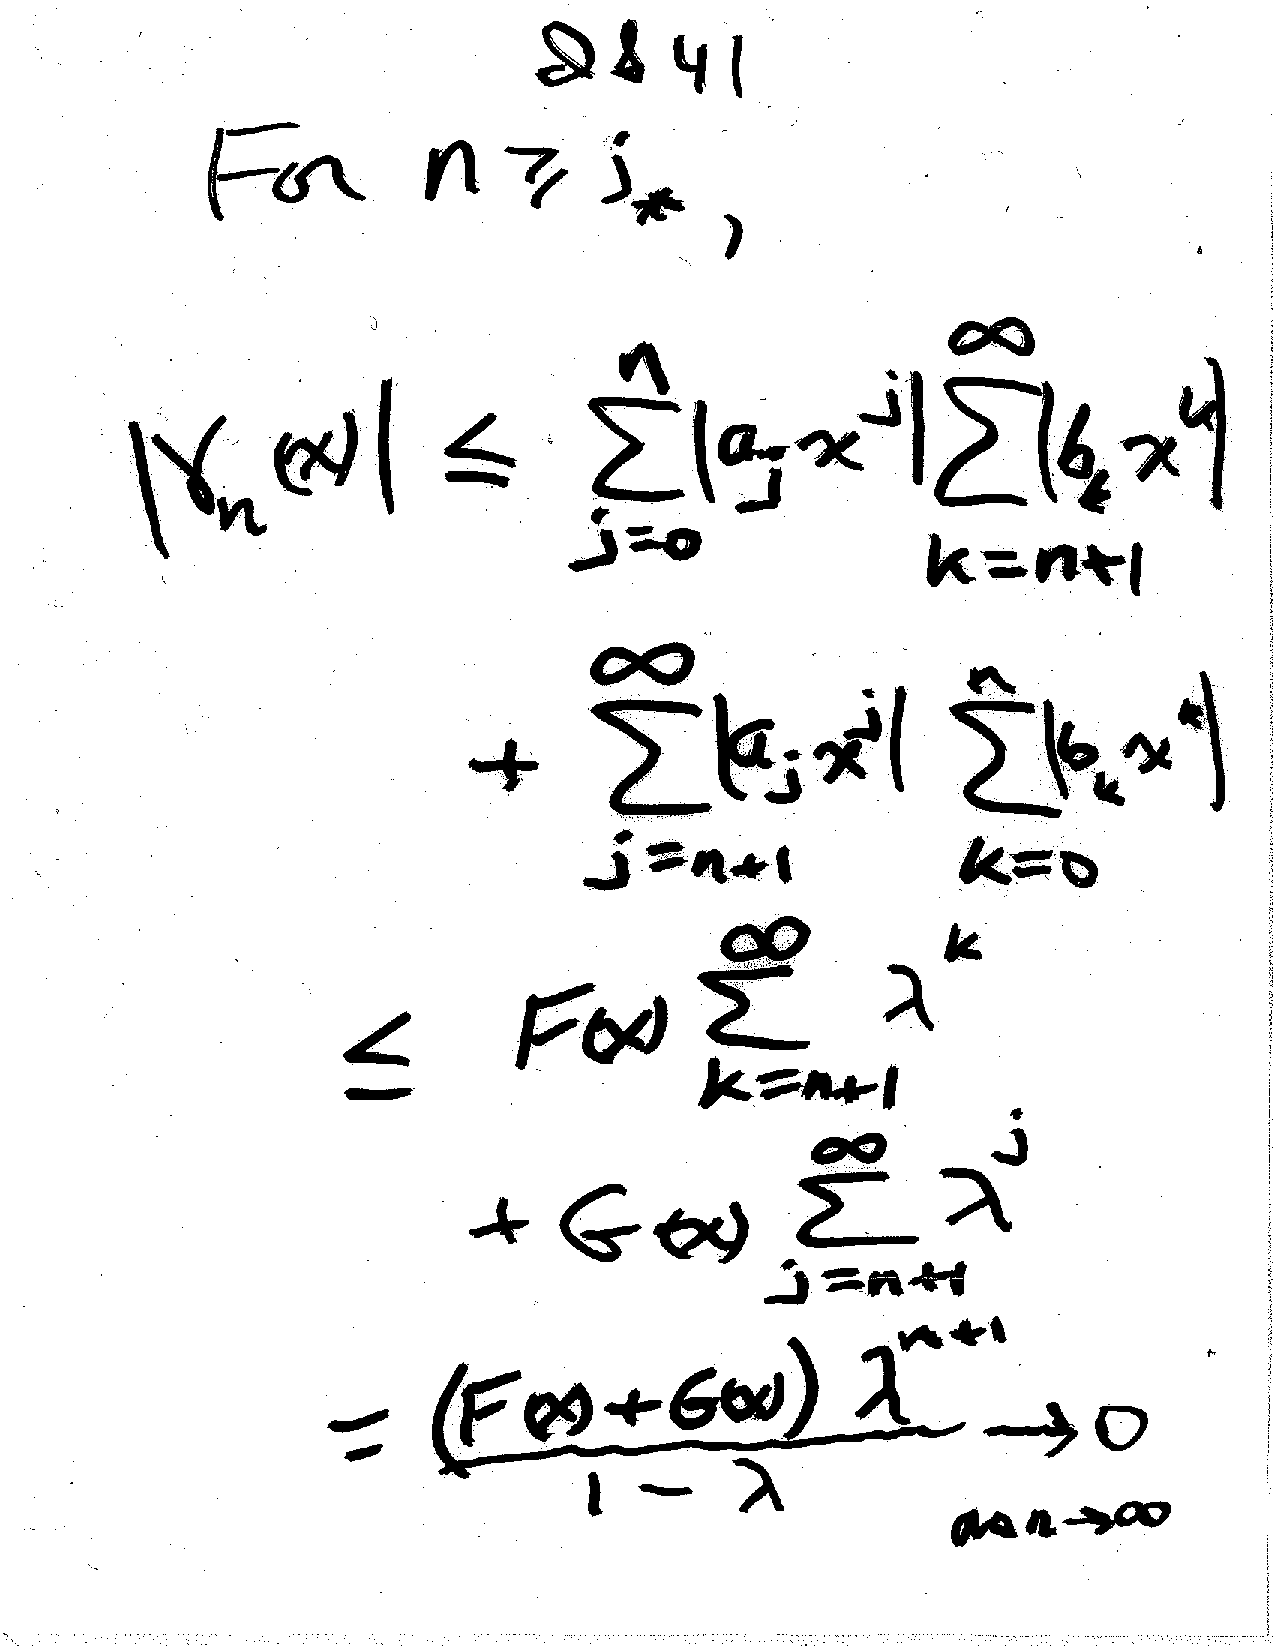
\includegraphics[scale=.5]{Pages/IS_41}

\newpage

Therefore $$ h_n (x) - \tilde{h}_n (x) \rightarrow 0$$
so 
$$h (x) = \lim_{n \rightarrow \infty} \tilde{h}_n (k)$$
$$= \sum_{n=0}^\infty (\sum_{j=0}^n a_jb_{n-j})x^n$$

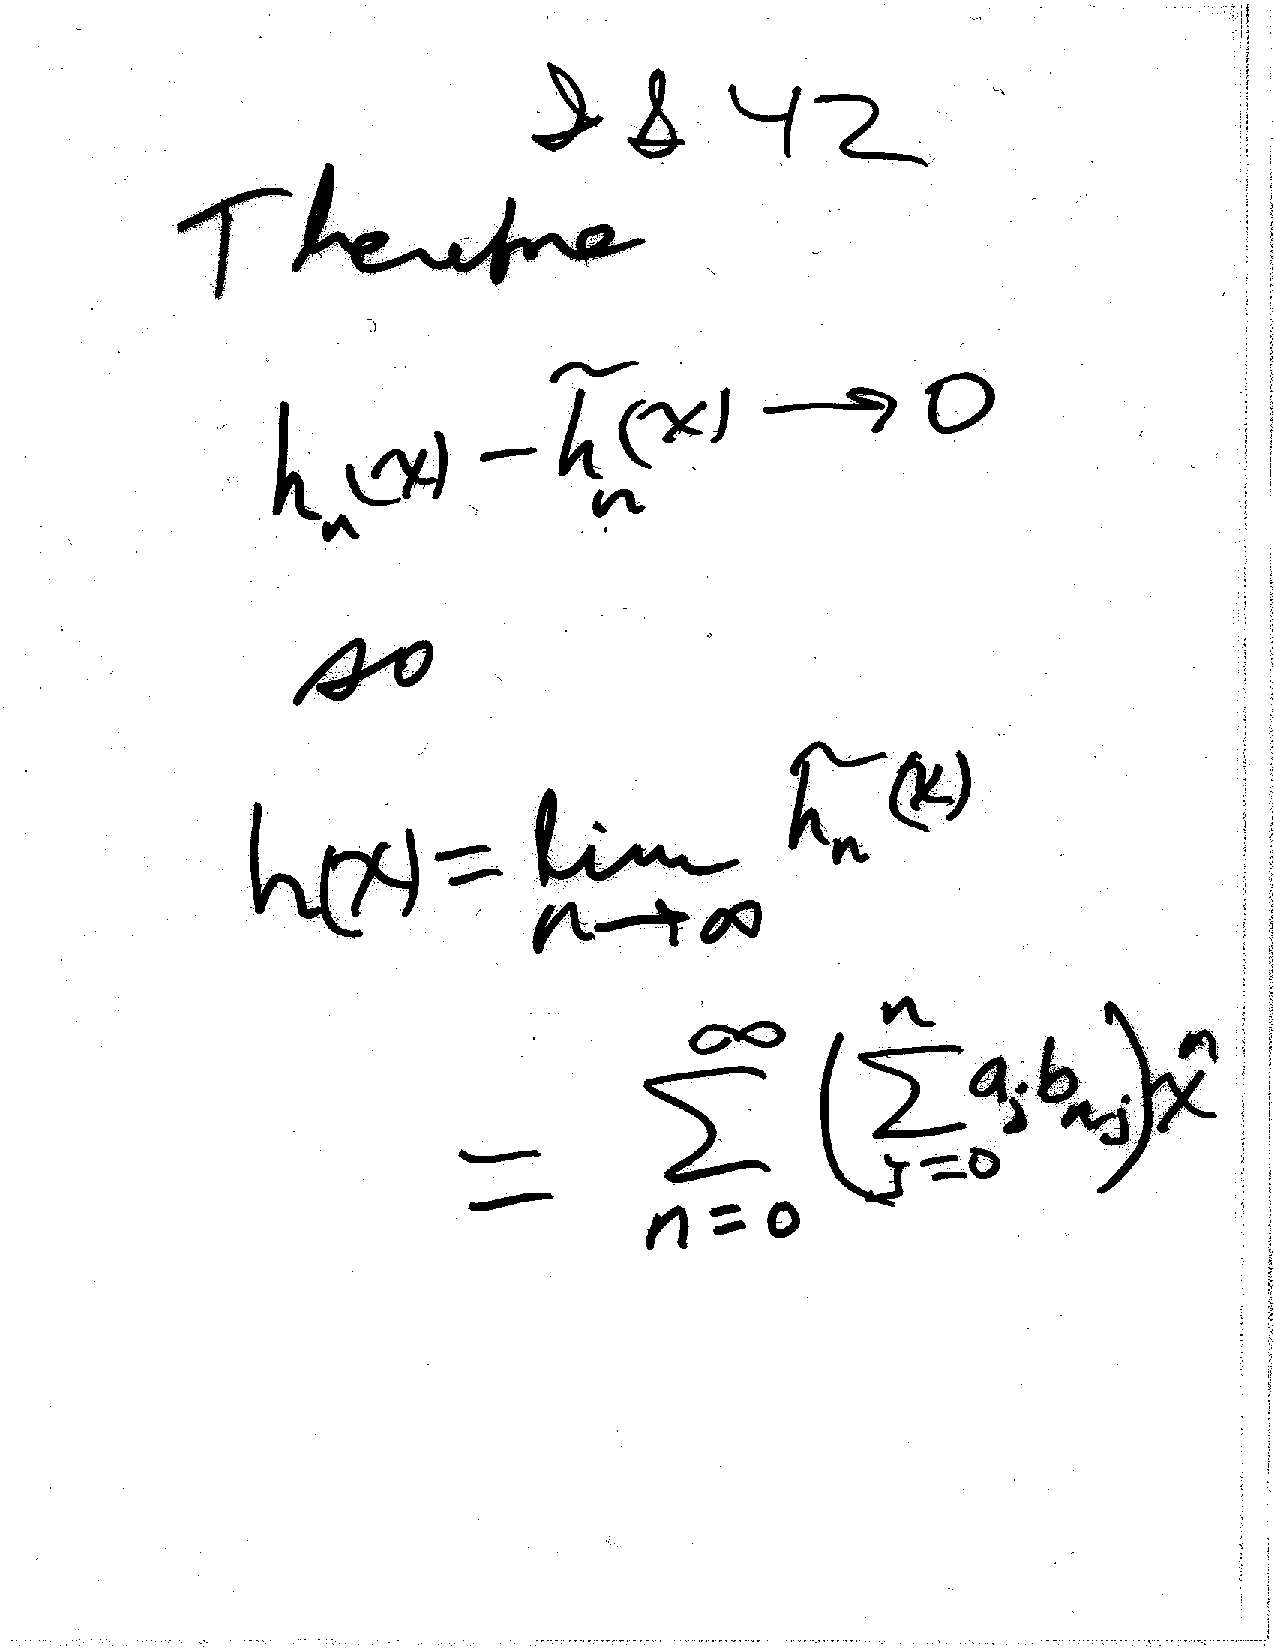
\includegraphics[scale=.5]{Pages/IS_42}


\section{Metric Spaces Part 2}


%Bryant: M1-M7

%Reshma: M8-M14

%Ethan: M15-M21





\end{document}